%% PAPER design system v1.0.0 -- two-column paper (canonical house template).
%% Spec: ~/.claude/design/paper/PAPER.md. Compile: tectonic kraken_whitepaper.tex

\documentclass[10pt,twocolumn]{article}

\usepackage[utf8]{inputenc}
\usepackage[T1]{fontenc}
\usepackage{times}
\usepackage[margin=1.9cm,columnsep=0.65cm,top=1.7cm,bottom=2.0cm]{geometry}
\usepackage{titlesec}
\usepackage{booktabs}
\usepackage{array}
\usepackage{graphicx}
\usepackage{amsmath}
\usepackage{caption}
\usepackage[hidelinks,colorlinks=false]{hyperref}
\usepackage{fancyhdr}
\usepackage{enumitem}
\usepackage{xcolor}
\usepackage{microtype}
%% Reduce loose interword spacing in narrow two-column justified text (XeTeX
%% has no font expansion, so use protrusion + a generous emergencystretch and
%% let TeX hyphenate a little more aggressively to find better breaks).
\microtypesetup{protrusion=true}
%% Interword spacing: ragged-right keeps word spaces uniform and tight in narrow
%% two-column text (XeTeX cannot do pdftex font expansion, and justified narrow
%% columns stretch spaces unevenly). ragged2e keeps hyphenation, so the right edge
%% stays only lightly ragged; paragraph indent is preserved.
\usepackage[document]{ragged2e}
\hyphenpenalty=50
\emergencystretch=1em
\usepackage{seqsplit}
\usepackage{pifont}
\usepackage{fancyvrb}
\usepackage{tcolorbox}
\tcbuselibrary{breakable}

%% Palette: professional black and white only, no green accent.
\definecolor{inkblack}{HTML}{1A1A1A}
\definecolor{hair}{HTML}{9A9C9F}
\definecolor{notebg}{HTML}{F2F2F2}

\newcommand{\cmark}{\ding{51}}
\newcommand{\xmark}{\textcolor{hair}{\ding{55}}}
\newcommand{\wmark}{\textbf{\ding{51}}}

\setlength{\parindent}{1em}
\setlength{\parskip}{0pt}
\captionsetup{font=small,labelfont=bf,skip=4pt}

%% Float packing: keep figures near their references; allow full-width floats at bottom.
\usepackage{stfloats}
\renewcommand{\topfraction}{0.92}
\renewcommand{\bottomfraction}{0.85}
\renewcommand{\textfraction}{0.06}
\renewcommand{\floatpagefraction}{0.72}
\renewcommand{\dbltopfraction}{0.92}
\renewcommand{\dblfloatpagefraction}{0.72}
\setcounter{topnumber}{3}
\setcounter{bottomnumber}{2}
\setcounter{totalnumber}{5}
\setcounter{dbltopnumber}{3}

\titleformat{\section}{\normalfont\large\bfseries}{\thesection.}{0.6em}{}
\titleformat{\subsection}{\normalfont\bfseries}{\thesubsection.}{0.6em}{}
\titlespacing*{\section}{0pt}{10pt}{5pt}
\titlespacing*{\subsection}{0pt}{7pt}{3pt}

\pagestyle{fancy}
\fancyhf{}
\fancyfoot[C]{\footnotesize\thepage}
\renewcommand{\headrulewidth}{0pt}
\renewcommand{\footrulewidth}{0pt}

\newcommand{\kraken}{\textsc{Kraken}}
\newcommand{\code}[1]{\seqsplit{\texttt{#1}}}

\newtcolorbox{finding}[1]{breakable,colback=notebg,colframe=inkblack,boxrule=0.8pt,
     arc=1.5pt,left=7pt,right=7pt,top=4pt,bottom=4pt,
     title={\small\bfseries #1},coltitle=black,colbacktitle=notebg,fonttitle=\bfseries}

%% House two-column title block: title between black rules.
\makeatletter
\renewcommand{\@maketitle}{%
  \vspace*{-1em}
  {\noindent\rule{\textwidth}{1pt}\par\vspace{0.35em}}
  {\centering\bfseries\Large Kraken: A Cascade CTF-Autosolver\par\vspace{0.35em}}
  {\noindent\rule{\textwidth}{0.5pt}\par\vspace{0.7em}}
  {\centering Jackson Stephens\par}
  {\centering\small project\_kraken \;\textbullet\; jackson@stephens.sh \;\textbullet\; July 2026 \;\textbullet\; Technical Report \;\textbullet\; v0.2.5\par}
  \vspace{0.5em}
}
\makeatother
\title{}\author{}\date{}

\begin{document}
\twocolumn[
  \begin{@twocolumnfalse}
    \maketitle
    \begin{abstract}
    \noindent
    \kraken{} is a capture-the-flag (CTF) auto-solver whose guiding principle is that tools produce
    artifacts that language models can then reason about. Rather than invoking the model at every step
    and stage of the problem-solving path, that is, rather than tossing a challenge binary and its
    description at a language model and hoping, \kraken{} routes each challenge through a cheapest-first
    \emph{cascade} that tries to find the flag with deterministic tooling and no model call at all,
    escalating to model reasoning only when computation runs out. A deterministic validator is the sole
    oracle, so the system never reports a hallucinated flag as a win; a closed-loop optimizer learns
    from every solve and re-orders the cascade so that winning tools run first. The graph is a
    model-agnostic harness: it can run offline on a local model, and in practice drives frontier models
    through Claude Code with a Codex agentic rescue seat for the hard tail. This report is a full account
    of the system: a 20-node LangGraph engine, twelve classification labels routed to nine specialist
    subgraphs, a library of 85 registered helper tools (about 59k lines), a validator with seventeen
    flag-format patterns and hallucination guards, a manager with eight deterministic anti-thrash guards,
    a self-improving optimizer, a 30-tool MCP server, live-competition autopilot, and a full
    attack-defense tick engine that both mass-throws exploits and self-heals its own services. It is
    backed by 1{,}037 tests and a great deal of experimentation. I document what works and what does not,
    in the agent's own words: a hands-off clear of every online-solvable challenge at BYU EOS CTF, a run
    at KalmarCTF whose \texttt{flag\_checker} solve recovered a flag whose author had written his
    disbelief that an AI could solve it, and a sub-ten-minute breakdown of an embedded attack-defense
    firmware target at MITRE eCTF, closing with an honest assessment of the pitfalls that lead into the
    future work and the improvements they point to.
    \end{abstract}
    \vspace{0.7em}
  \end{@twocolumnfalse}
]

\section{Introduction}

A capture-the-flag challenge has a binary success metric. You either solve it or you do not; you win or
you lose. There is no partial credit and no talking your way to a better grade. That harsh, all-or-nothing
verdict, sitting at the end of the complex, multi-step work it takes to actually reach a flag, is what
makes CTF an unusually ideal testbed in the pursuit of a vulnerability-research agent to augment cyber
operations. It is also a domain where a large fraction of the real work is \emph{computation} rather than
open-ended reasoning: disassembling a binary, brute-forcing a weak cipher, walking a constraint system
through a solver, carving a file, matching a libc build from a leaked address.

Most published CTF agents put a language model in the loop at every step. That is flexible and, on the
hardest challenges, necessary. It is also slow, non-deterministic from run to run, and, on a hosted
frontier model, expensive per challenge. \kraken{} takes the opposite default. Its guiding principle, and
the one thing to take away if you take away nothing else, is that \emph{tools produce artifacts that
language models can then reason about}: for the computational fraction of a CTF, which is most of it, a
model is not merely unnecessary but a liability, because it injects latency, cost, and variance into a
step a deterministic tool finishes correctly and repeatably. So \kraken{} inverts the usual arrangement.
It is an ensemble, an engine, a harness of intelligence: it tries to solve each challenge with tooling and
no model call, and reaches for the model last, as the thing that guides the harness rather than the thing
that does every step. I built the core during Opus 4.5, validated it through 4.6, and the last competition
it ran used 4.7, and part of what that arc taught me is that the frontier was moving underneath the
project (Section~\ref{sec:future}).

This report is long on purpose. \kraken{} is not a single script; it is an ensemble of many parts, and
the earlier short writeups did it a disservice by compressing a large system into a teaser. Here I document the
whole thing: the graph and its nodes (Section~\ref{sec:graph}), classification and the total route
map (Section~\ref{sec:routing}), the nine specialists (Section~\ref{sec:specialists}), the tool
router and cascade (Section~\ref{sec:router}), the 85-tool library (Section~\ref{sec:library}), the
solve engine (Section~\ref{sec:solve}), the validator oracle (Section~\ref{sec:validator}), the
manager and its eight guards (Section~\ref{sec:manager}), the learned-experience optimizer
(Section~\ref{sec:learn}), the model layer and the Codex rescue seat (Section~\ref{sec:models}), the
attack-defense engine (Section~\ref{sec:ad}), the wider platform (Section~\ref{sec:platform}), and
the test suite (Section~\ref{sec:tests}). Then the value: what \kraken{} actually did, in the agent's
own words (Section~\ref{sec:practice}), the honest evaluation (Section~\ref{sec:eval}), the
significance beyond CTF (Section~\ref{sec:impact}), the lessons (Section~\ref{sec:lessons}), and the
roadmap (Section~\ref{sec:future}). A complete tool catalog is in Appendix~\ref{sec:appendix}.

\medskip
\textbf{A request, before anything else.} For the sake of the competitions themselves: please do not use
work like this to poison the legitimacy of other teams or their ability to compete at the highest level,
simply for the bragging rights. Capture-the-flag is, for most people, the
introduction to vulnerability research. It is a proving ground and a rare chance to both showcase real
skill and compete at the very top of a niche corner of security. Third-partying your way through a
competition in pursuit of something that is, arguably, against the entire nature of the competition takes
that opportunity away from the people it is meant for, and in my opinion that is wrong. So I ask sincerely:
if you plan to emulate the findings and architecture of this paper, please do so responsibly. And if you
point the system at a live CTF, please ask to be removed from the leaderboard, or don't. I can't really tell
you what to do. I just ask that you think about it, for the sake of the competition space.

\subsection*{Contributions and scope}

\begin{itemize}[leftmargin=1.1em,itemsep=1.5pt,topsep=2pt]
\item A cheapest-first, \emph{model-last} cascade, an ensemble of deterministic tooling that resolves
the static majority of CTF challenges with no model call.
\item A \emph{total} classification-and-routing scheme with a deterministic validating oracle, so
autonomy is safe: no class is ever stranded, and a non-flag is never reported as a solve.
\item A learned-experience optimizer that reorders the cascade from past solves and emits an auditable
configuration rather than an opaque weight update.
\item An expansion from jeopardy solving into full attack-defense play, both throwing exploits across
a field of teams and defending and self-healing one's own services.
\item An honest account of where this design wins (static, structured challenges) and where it does
not (dynamic, interactive ones), backed by real competition results.
\end{itemize}
\noindent Out of scope, and deferred to its own documentation: the sister vulnerability-research
agent that shares \kraken{}'s case-state ledger, and the private per-challenge writeups and offline
benchmark harness that live in the development tree. That sister project, \texttt{project\_blackbox},
will have its own paper releasing soon, on how I used it to find my first zero-day.

\section{Related Work and Novelty}
\label{sec:related}

\textbf{The multi-agent line.} \kraken{} began as a from-scratch reimplementation of \emph{Squid
Agent} (SPL Team) \cite{squid2024}, which built on CSAW's \emph{D-CIPHER} planner and executor system
\cite{udeshi2025dcipher}. From that line I kept the idea that mattered most: \textbf{per-category
specialist agents}, mirroring how a real CTF team assigns a reverser, a pwner, and a crypto person.
D-CIPHER formalizes this as a Planner coordinating heterogeneous Executors and reports
state-of-the-art results in the low tens of percent on the full, uncurated benchmarks
\cite{udeshi2025dcipher}, a useful reminder of how hard the general problem is. EnIGMA
\cite{abramovich2025enigma} showed that giving an agent genuine interactive tools (a live debugger, a
persistent connection) substantially helps, a result that predicts exactly where \kraken{} later fell
short (Section~\ref{sec:lessons}). HackSynth \cite{muzsai2024hacksynth} pairs a Planner and a
Summarizer for autonomous penetration testing. Every one of these keeps a model in the loop
throughout.

\medskip
\textbf{The model-racing line.} A newer and different approach is VeriLabs' CTF agent
\cite{verialabs2026}, which won BSidesSF~2026 with a 52/52 clear by \emph{racing multiple frontier
models in parallel}. A coordinator dispatches solver swarms, each running several models at once (for
example Claude Opus, GPT-5.4, and GPT-5.3-codex) in isolated Docker containers, and the first to find
a flag wins; the solvers ``never give up.'' This is a powerful and expensive strategy: it maximizes
solve rate by maximizing frontier-model throughput.

\medskip
\textbf{Where \kraken{} differs.} The difference is one of posture, not scorecard (Table~\ref{tab:novelty}).
Both prior lines put the model at the center: D-CIPHER runs one in the loop at every step, and VeriLabs
races several at once. \kraken{} puts the \emph{harness} at the center and the model at the edge. The
solve is carried by an ensemble of deterministic tooling, and a model is called last, to guide the
harness when the tooling runs out rather than to perform each step. Because the tooling and the routing
live in the harness rather than in a particular model, the same system runs on a local model or a
frontier one; it is model-agnostic by construction (Section~\ref{sec:models}). Two things follow that
the other lines do not build in: a \textbf{learned-experience optimizer} (Section~\ref{sec:learn}) that
tunes the ensemble from past solves, and first-class \textbf{attack-defense} play (Section~\ref{sec:ad}).
I make no claim that the other systems cannot reproduce a solve, run offline, or specialize by category;
those are not the axis. The axis is where the intelligence sits and what carries the work.

\begin{table}[t]
  \centering\small
  \setlength{\tabcolsep}{6pt}\renewcommand{\arraystretch}{1.3}
  \setlength{\tabcolsep}{4pt}
  \begin{tabular}{@{}l ccc@{}}
    \toprule
    & \textbf{Squid/} & & \\[-2pt]
    & \textbf{D-CIPHER} & \textbf{VeriLabs} & \textbf{\kraken{}} \\
    \midrule
    Model use   & Every step & Racing   & \textbf{Last resort} \\
    Carried by  & the model  & the race & \textbf{the tools} \\
    Learns      & \xmark     & \xmark   & \wmark \\
    \bottomrule
  \end{tabular}
  \caption{The axis that matters: where the intelligence sits and what carries the solve. This is a
  statement of design posture, not a scorecard of what the other systems are capable of.}
  \label{tab:novelty}
\end{table}

\section{System Overview}
\label{sec:overview}

\kraken{} is a LangGraph \code{StateGraph} of roughly 20 nodes over a \code{KrakenState} TypedDict of
about 48 fields. It runs in several modes from one core (Section~\ref{sec:platform}): a standalone
solver over a challenge directory, a live-competition autopilot that pulls from and submits to CTFd, a
batch \code{solve-all} runner, an MCP server that exposes the deterministic tooling to an external
agent such as Claude Code, a FastAPI browser GUI, and an attack-defense engine. Underneath sits a
library of 85 registered helper scripts (about 59k lines across roughly 100 files on disk), sequenced
by a deterministic router.

Three ideas recur throughout and are worth stating once. First, \textbf{tiering}: every node is
tagged deterministic, LLM-low, LLM-mid, or LLM-high, and the design goal, stated in the graph module
itself, is that ``the happy path uses 0 Opus tokens.'' Second, \textbf{the oracle}: only a
deterministic validator can confirm a flag, so the model may propose but never certify. Third,
\textbf{totality}: every routing decision has a defined fallback, so a novel or misclassified
challenge is never stranded. The rest of this report is those three ideas worked out in detail.

\section{The Processing Graph}
\label{sec:graph}

\subsection{The cascade}

Every challenge descends a four-tier cascade, cheapest first, and stops at the first tier that
produces a flag the deterministic validator accepts (Figure~\ref{fig:cascade}, Table~\ref{tab:tiers}).
The top tier is the load-bearing one: for a large class of challenges the flag falls out of
deterministic computation with no model call, which is what makes a sub-minute median and \$0
operation possible at all. Only when the tools stall does a model enter, first to write a targeted
solve script, then for interactive exploitation, and last for a heavyweight agentic fallback with full
shell access. Each tier carries an explicit time budget, and per-strategy timeouts keep any single
tool from eating the whole budget (Section~\ref{sec:router}).

\begin{figure}[t]
  \centering
  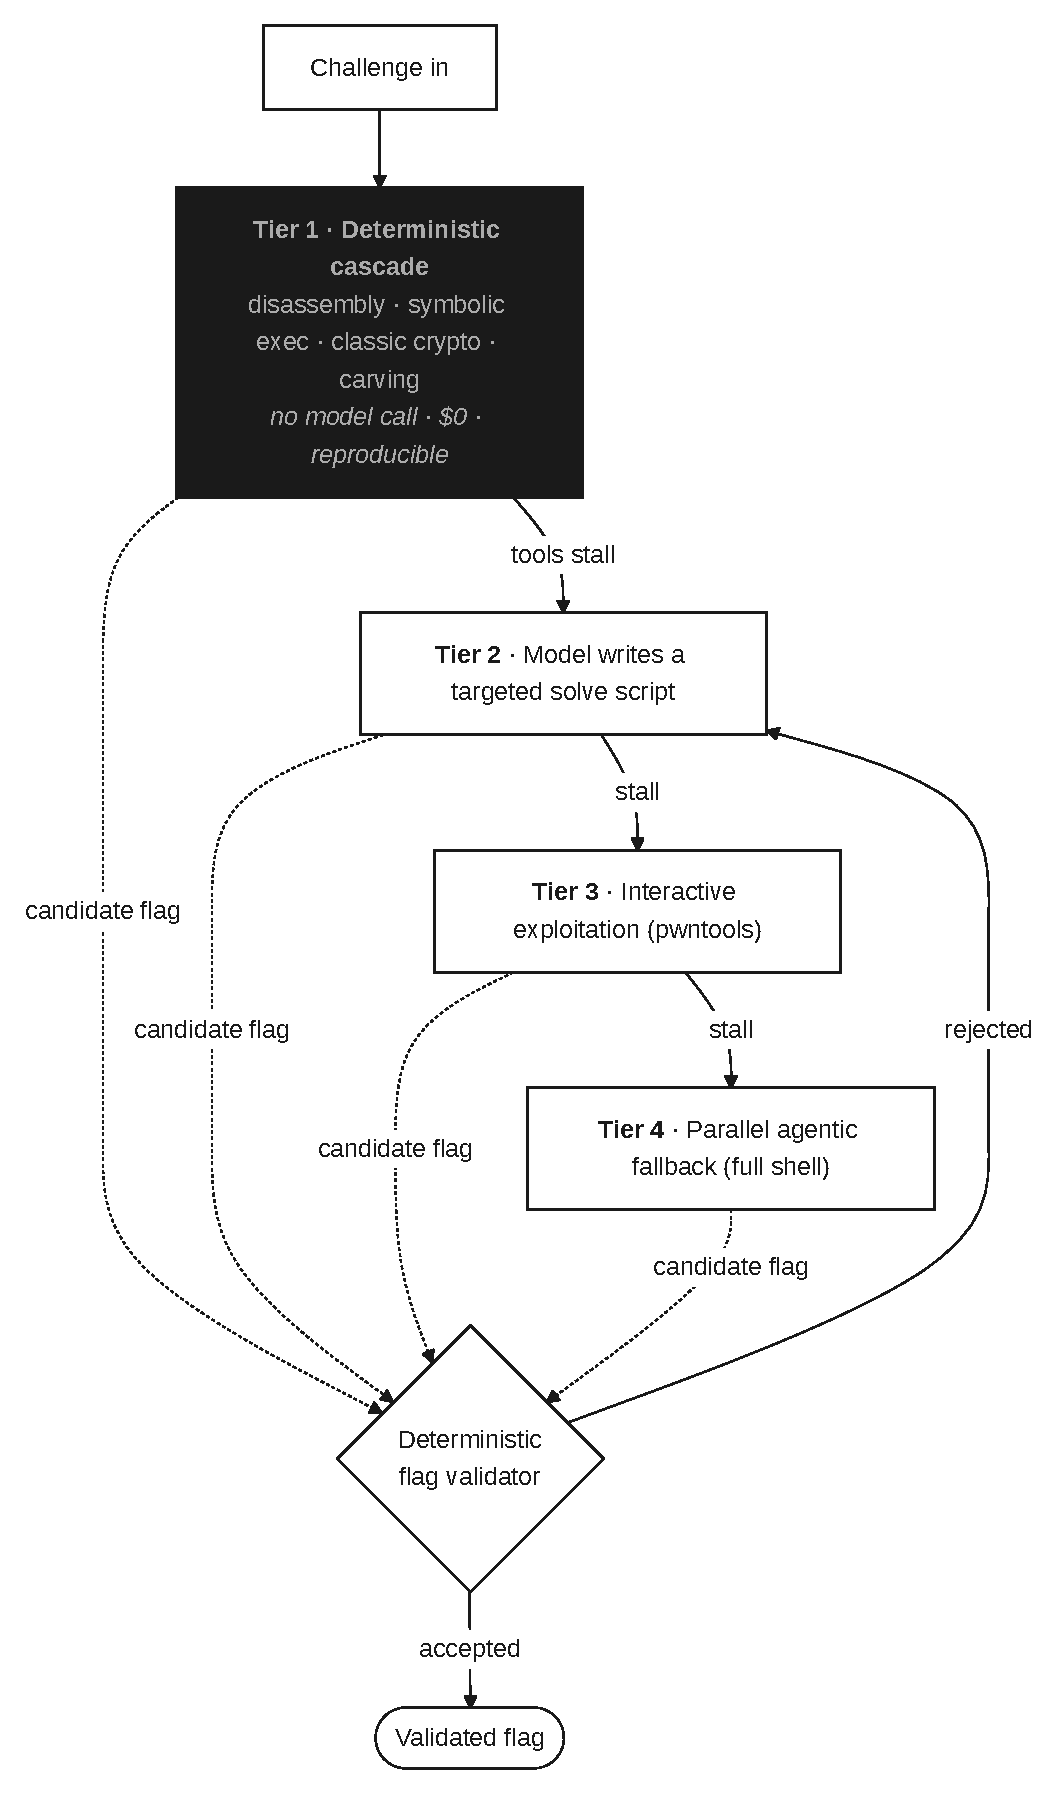
\includegraphics[width=0.86\linewidth]{figures/fig_cascade.pdf}
  \caption{The cheapest-first cascade. Each tier escalates only when its tools stall; a validated
  flag at any tier ends the run. The top deterministic tier (in black) resolves most static challenges with no model call, at zero
  cost, byte-for-byte reproducibly.}
  \label{fig:cascade}
\end{figure}

\begin{table*}[t]
  \centering\small
  \setlength{\tabcolsep}{6pt}\renewcommand{\arraystretch}{1.25}
  \begin{tabular}{@{}l l l l p{0.44\linewidth}@{}}
    \toprule
    \textbf{Tier} & \textbf{Budget} & \textbf{Model} & \textbf{Cost} & \textbf{What runs} \\
    \midrule
    1. Deterministic cascade & $\sim$30\,s  & none              & \$0   & the 85-tool helper library: decoders, symbolic execution, classic crypto, carving; most solves end here \\
    2. Model solve-script    & $\sim$120\,s & LLM-high          & paid  & the solve engine writes a targeted script the tools could not, with a generate/execute/fix loop \\
    3. Interactive exploit   & $\sim$300\,s & LLM-high          & paid  & a driven exploit or remote-service session for stateful challenges \\
    4. Agentic fallback      & $\sim$900\,s & LLM-high + Codex  & paid  & Codex gets full file access and no graph constraint; the once-per-challenge last resort \\
    \bottomrule
  \end{tabular}
  \caption{The four tiers, cheapest first. A validated flag at any tier ends the run; a higher tier
  fires only when the ones below it stall. Budgets are nominal timeouts. Tier~1 carries the large
  static body of a competition at zero model cost.}
  \label{tab:tiers}
\end{table*}

\subsection{Assembly, nodes, and the zero-Opus happy path}

The graph assembly, in \code{build\_graph()}, wires a linear intake pipeline, followed by a classification
branch and a convergence back onto the router. The spine is triage, unpack, decompile, normalize, and
classify. Classification then routes to one of nine specialist subgraphs, each of which edges to parameter
extraction and then to the tool router. The router either short-circuits to the validator (if the tool cascade already
found a flag) or hands off to the solve engine. The validator ends the run, self-corrects, or escalates
to the manager, which can route to any node or terminate. Table~\ref{tab:nodes} lists the principal
nodes and their tiers.

The design invariant, quoted from the graph module, is that ``the happy path uses 0 Opus tokens.
Manager only fires on failure. Tool router can short-circuit to \code{flag\_validator} without any LLM
call.'' Concretely, \code{route\_after\_tools} returns \code{flag\_validator} whenever the cascade set a
\code{tool\_flag\_candidate}, so the LLM solve engine is skipped entirely on a deterministic solve
(Figure~\ref{fig:nodes}).

\begin{figure*}[t]
  \centering
  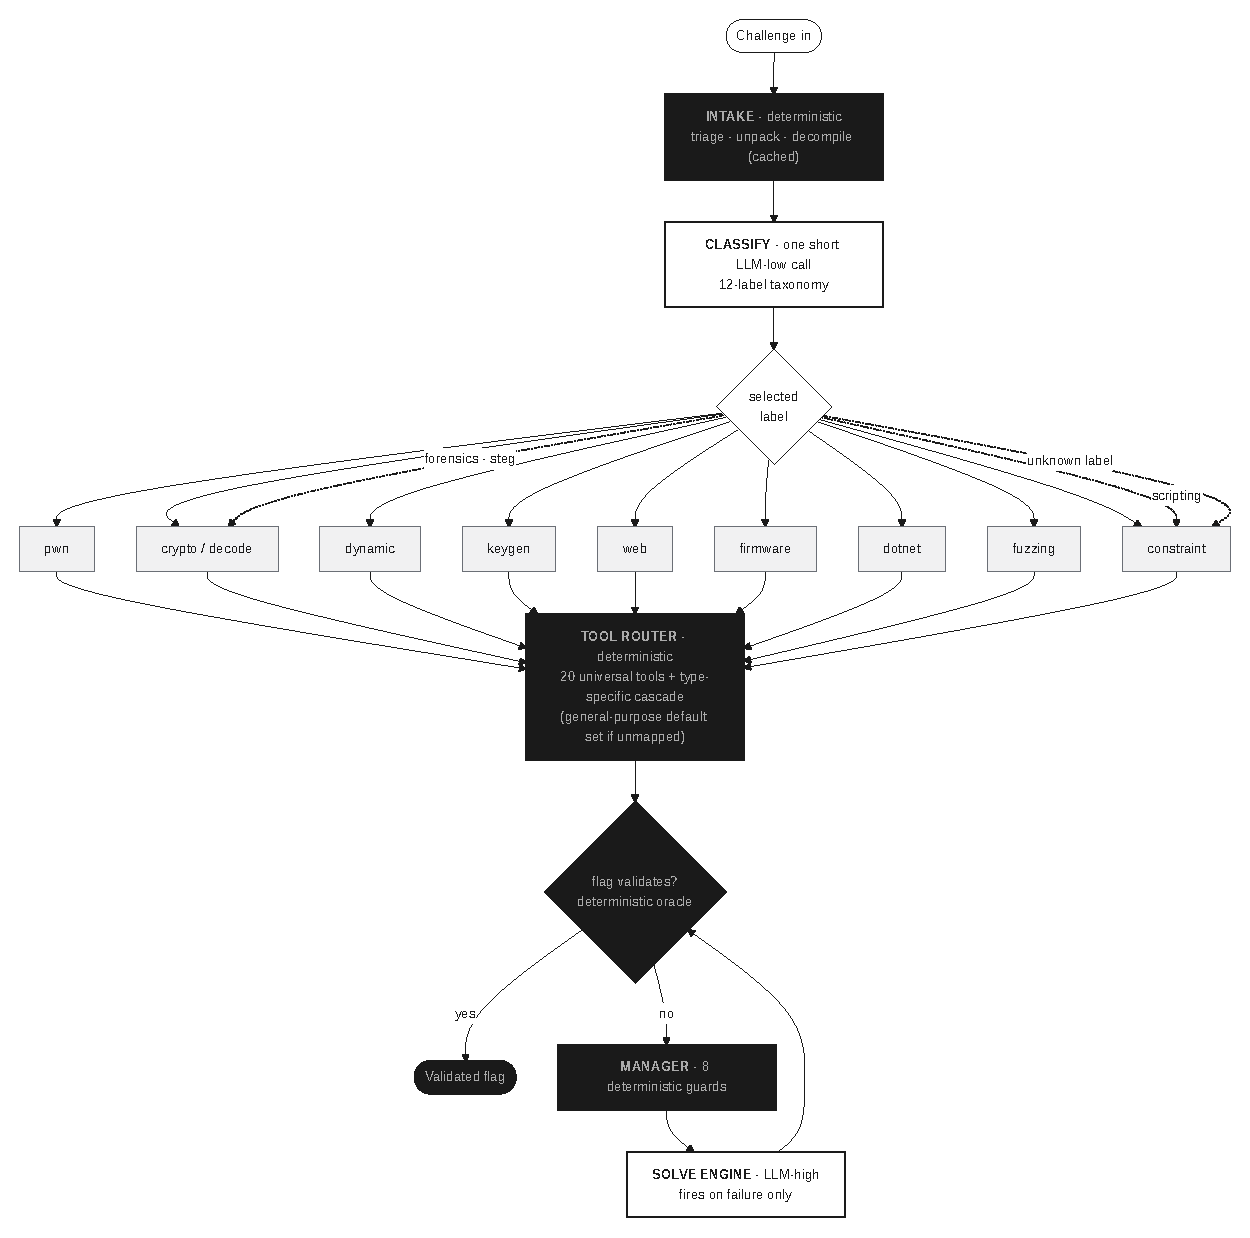
\includegraphics[width=0.94\linewidth]{figures/fig_nodes.pdf}
  \caption{Node selection for one solve. Classification emits one of twelve labels, routed to nine
  specialist subgraphs; several labels share a specialist (dotted), and any label the route map does
  not recognize falls back to the constraint solver, so no class is ever stranded. The deterministic
  path (in black) carries intake, the tool router, and the validating oracle. A model (white) is reached
  only for the one short classification call and, on failure, the solve engine.}
  \label{fig:nodes}
\end{figure*}

\begin{table*}[t]
  \centering\small
  \setlength{\tabcolsep}{6pt}\renewcommand{\arraystretch}{1.18}
  \begin{tabular}{@{}l l p{0.52\linewidth}@{}}
    \toprule
    \textbf{Node} & \textbf{Tier} & \textbf{What it does} \\
    \midrule
    \code{triage}          & deterministic  & auto-detect the artifact; runs \texttt{file}, strings, pwntools, and lief analyses concurrently; detects .NET, \texttt{.pyc}, Office macros, and remote services \\
    \code{unpack}          & deterministic  & a no-op unless packed; UPX decompress or dynamic-dump, then continues on the original if it fails \\
    \code{decompile}       & det.\ (cached) & headless Ghidra to C, with a pyelftools and capstone fallback; \texttt{.pyc}, .NET, and VBA-macro paths \\
    \code{normalize}       & LLM-low        & rename variables and add comments into an annotation store, never overwriting the decompilation \\
    \code{classify}        & LLM-low        & assign one of twelve labels, with a keyword-scoring heuristic fallback when the model is unavailable \\
    \code{constraint\_solver} & subgraph    & pure angr and z3; also the routing fallback for unrecognized labels \\
    \code{crypto\_decode}  & subgraph       & cipher detection and a cascade of decoders (base64, hex, XOR sweep, encrypted shared libraries) \\
    \code{pwn\_specialist} & tools + LLM    & vulnerability indicators, ROP gadgets, buffer sizes, \texttt{/bin/sh} strings \\
    \code{web\_specialist} & LLM-mid        & framework and vuln-class detection (SQLi, SSTI, SSRF, deserialization), route extraction \\
    \code{fuzzing\_specialist} & LLM-mid    & entry-point ranking and AFL++ or libFuzzer harness generation \\
    \code{dotnet\_specialist} & no LLM      & installs mono, ilspycmd, monodis; probes and hands the solve engine exact commands \\
    \code{firmware\_specialist} & LLM-mid   & binwalk, architecture detection, hardcoded-credential scan; embedded-target indicators \\
    \code{param\_extraction} & deterministic & sixteen solve parameters from decompilation by regex and heuristics (input mode, success string, ...) \\
    \code{tool\_router}    & deterministic  & sequences the 85-tool cascade with per-type timeouts; short-circuits on a validated flag \\
    \code{flag\_validator} & deterministic  & seventeen flag-format patterns, entropy and noise heuristics, hallucination detection: the oracle \\
    \code{solve\_engine}   & LLM-high       & codegen with a generate, execute, fix inner loop, auto-pip-install, and false-positive detection \\
    \code{manager}         & LLM-high       & failure router; runs eight deterministic guards before any model call \\
    \bottomrule
  \end{tabular}
  \caption{Principal nodes and their tiers. The deterministic and cached tiers (most of the table)
  carry a full solve on their own for the static majority; only the solve engine and manager are
  LLM-high, and they fire on failure. On the offline static subset the median solve never touches an
  LLM tier at all.}
  \label{tab:nodes}
\end{table*}

\subsection{Crash resilience and caching}

Two wrappers applied to every node make an unattended run survivable. \code{\_safe\_node} catches any
unhandled exception, logs it, increments a \code{framework\_crash\_count}, and reroutes to the manager;
for a solve-engine crash it synthesizes a failure attempt so the validator still has concrete input and
output to reason about. After eight cumulative crashes it hard-brakes to a clean termination, so one
misbehaving tool can never hang or crash a run. \code{\_cached\_node} wraps \code{triage} and
\code{decompile}: if the cache fields are already present in state, the node returns a no-op instead of
re-running, so expensive work like Ghidra decompilation never runs twice when the manager loops back.

\section{Classification and Routing}
\label{sec:routing}

Classification assigns one of twelve labels: constraint, crypto, dotnet, dynamic, keygen, pwn, fuzzing,
web, firmware, scripting, forensics, and steg. The primary path is a single short LLM-low structured
call; when the model is unavailable a deterministic keyword-scoring heuristic classifies instead, with
file-extension boosts (a \texttt{.pcap} favors forensics, an image favors steg). A deterministic route
map then sends each label to one of nine specialist subgraphs.

Two properties matter. First, several labels share a specialist by design: forensics and steg both
route to the crypto and decode specialist, because for those categories the helper tools do the real
work and the specialist only coordinates them, and scripting routes to the constraint solver. Second,
and more importantly, the route map is \emph{total}: any label it does not recognize, including a novel
or misclassified one, falls back to the constraint solver, the most general analysis specialist. The
tool router applies the same principle one level down: if a class has no dedicated tool cascade it uses
a general-purpose default set (symbolic execution via \texttt{angr}, a Z3 decompiler, gdb comparison and
solve helpers, a dynamic tracer, a deobfuscator, and a binary patcher), and the twenty universal tools
run for every challenge regardless of class. Misrouting is therefore rarely fatal; a wrong label costs
some time, not the solve.

\section{The Specialists}
\label{sec:specialists}

The nine specialists are where category expertise lives. Six are LLM-mid subgraphs that pair a
deterministic pre-pass with a single mid-tier model call; three are fully deterministic. Every
LLM-backed specialist emits fenced JSON that is parsed into a strategy hypothesis for the downstream
solve engine.

\medskip
\textbf{Constraint solver} (deterministic, subgraph). No LLM. It scans symbols and decompiled code for
success indicators (\texttt{correct}, \texttt{success}, \texttt{flag}, \texttt{win}) and failure words,
resolves PLT addresses with pwntools, and runs three angr strategies in order: address-based find,
string-based trace with veritesting, and a PLT-based search using \texttt{strcmp} as the target, over
stdin lengths of 32, 64, 128, and 256 bytes.

\medskip
\textbf{Crypto decode} (LLM-mid, subgraph). It identifies crypto imports by keyword, pulls constants,
rodata keys, and high-entropy sections, and runs an encoding-chain detector (base64, then hex, then a
XOR sweep over keys 1 to 255). It recognizes \texttt{dlopen}/\texttt{dlsym} patterns and hints that a
high-entropy custom section may be an encrypted shared library to load via ctypes.

\medskip
\textbf{Pwn specialist} (tools + LLM-mid). Its deterministic pre-pass flags dangerous functions
(\texttt{gets}, \texttt{scanf}, \texttt{strcpy}, \texttt{sprintf}, \texttt{memcpy}), infers a vulnerability
class (buffer overflow, format string, a ROP candidate when NX is set and no canary is present, a heap
candidate), extracts stack buffer sizes by regex, and produces gadget hints.

\medskip
\textbf{Web specialist} (LLM-mid). It parses challenge source rather than a binary, detecting language
and framework (Flask, Django, Express, PHP), vulnerability indicators (code injection, SSTI, SQLi, XSS,
deserialization, command injection, path traversal), auth mechanisms, and route endpoints.

\medskip
\textbf{Fuzzing specialist} (LLM-mid). It classifies input, parsing, and dangerous-sink functions,
computes a complexity score, and ranks up to five entry candidates; the model then chooses a harness
type (AFL persistent, libFuzzer, stdin, file, or network) with a seed corpus and dictionary.

\medskip
\textbf{Dotnet specialist} (no LLM). It auto-installs mono and the decompilers ilspycmd and monodis,
probes what is available, attempts a short execution, and writes explicit tool guidance so the solve
engine knows exactly which invocations to use.

\medskip
\textbf{Firmware specialist} (LLM-mid). It runs binwalk, architecture detection, and a
hardcoded-credential scan, and keyword-matches filesystem, bootloader, OS, and hardware indicators
(u-boot, squashfs, busybox, UART, JTAG) to flag embedded targets.

\medskip
\textbf{Keygen} (LLM-mid) is the smallest specialist, prompting for input format, transformations, and
the comparison target. \textbf{Dynamic analysis} (no LLM) patches anti-debug traps with lief, runs
differential input tracing, extracts encrypted data, and finishes with a string-guided angr trace. When
parallel specialists are enabled, a fan-out node runs the primary plus up to two secondary specialists
concurrently and merges their results, preferring the longest hypothesis and any satisfiable angr
result.

\section{The Tool Router and the Cascade}
\label{sec:router}

The router is the deterministic heart of the system. For a classified challenge it builds an ordered
cascade of tool names, all twenty universal tools first and then the type-specific bucket, resolves each
name to a concrete shell command, runs the commands one at a time, and scans their output for a flag.

\medskip
\textbf{Per-type budgets.} A base timeout is keyed on the challenge type: 60 seconds for crypto and
keygen; 90 for constraint, dynamic, steg, and scripting; 120 for pwn, fuzzing, web, firmware, and
forensics; 180 for miscellaneous and blockchain; 300 as the floor for any remote tool. The constraint
timeout carries a revealing code comment, ``was 300 -- \texttt{auto\_angr} can eat entire budget'': the
number is the residue of a real failure (Section~\ref{sec:lessons}).

\medskip
\textbf{Command builders are precondition gates.} Each tool name resolves through one of about fifty
custom builder functions (or a generic directory-flag or binary-flag builder). Crucially, a builder
returns nothing, and the tool is skipped, when its precondition is not met: the steg builder requires an
image, the pcap builder requires a capture file, the patcher fires only when a flag-gate or no-input mode
is suspected, and the angr builder requires a discovered success string. This is how a nominal cascade of
two dozen tools collapses to the handful actually applicable to a given challenge, at zero model cost.

\medskip
\textbf{Execution and the flag contract.} Each command runs as a shell subprocess in its own process
group, so on timeout the entire tree is killed (important because angr and z3 spawn children). Output is
scanned by a precedence chain: an explicit \texttt{EXTRACTED FLAG:} marker first, then the challenge's
flag-format regex, then generic patterns, then incomplete-flag repair (reconstructing a flag that crashed
before printing its closing brace), then prefix-wrapping of a bare body. Candidates are filtered against
runtime noise, shell expressions, and code fragments, and a repetitive single-character body is rejected
as a false positive without stopping the cascade. The uniform contract is what makes the library
hot-pluggable:

\begin{Verbatim}[frame=single,fontsize=\small,framesep=4pt,samepage=true]
$ auto_steg_extract.py challenge.png
[+] LSB scan ............. skip
[+] color-plane split .... skip
[+] appended-data carve .. HIT
EXTRACTED FLAG: flag{h1dd3n_in_the_p1x3ls}
\end{Verbatim}

\noindent A line matching \texttt{\textasciicircum{}EXTRACTED FLAG:} on exit code zero is a solve; any
nonzero exit means no flag, and the router moves to the next helper. On a hit it short-circuits the
cascade and hands the candidate to the validator.

\medskip
\textbf{Sequential by design.} The cascade is a single loop with no cross-tool parallelism; the only
concurrency is inside a tool's own subprocess. This is deliberate. A deterministic, sequential cascade is
reproducible and cheap to reason about, and the cheapest-first ordering means the expensive tools rarely
run. Remote tools are appended only when a live service is present, and for pwn the timing-attack tool is
stripped because network jitter produces false positives. A special case retries \texttt{angr} in
argv-input mode when its stdin run reports unsat or a timeout.

\section{The Tool Library}
\label{sec:library}

Underneath the router is the library that does the work: about 100 standalone \code{auto\_*.py} helper
scripts (roughly 59{,}000 lines in total), of which 85 are registered and routable through a single
\code{tool\_meta.json} manifest (Figure~\ref{fig:taxonomy}). Twenty \emph{universal} tools run for every
challenge, in a fixed order (source decoding, constraint extraction, static run, archive and git search,
QR and maze solvers, hash cracking, PDF and PCAP extraction, steg extraction, file carving, classical
ciphers, and a bash-solver runner). The rest are \emph{type-specific}, organized into fourteen categories
(Table~\ref{tab:categories}), plus five remote tools for networked services. The tool categories are a
superset of the twelve classifier labels: blockchain and attack-defense are tool families the router can
draw on without being primary classification classes of their own.

A handful of helpers carry a disproportionate share of the solves (Table~\ref{tab:helpers}). The largest,
\code{auto\_pwn\_solve} (about 73k bytes), bundles thirteen exploit strategies tried in order: direct
execution, ret2win, ret2shellcode, format-string GOT overwrite, ret2libc, ROP chain, stack pivot,
one-gadget, ret2dlresolve, SROP, ret2csu, PIE partial overwrite, and canary brute-force. A complete
catalog is in Appendix~\ref{sec:appendix}.

The library is also how the system grows from experience. When a challenge is genuinely new and the cascade
has no tool for it, the solve engine writes a one-off script to crack it (Section~\ref{sec:solve}); the good
ones do not stay one-off. A script that solves a novel class gets cleaned up into a standalone
\code{auto\_*.py} helper, registered in \code{tool\_meta.json}, documented, and slotted into the right category,
so the next challenge of that shape is handled by the cheap deterministic tier instead of re-deriving the
solution with a model. This is the same loop the firmware category came from (Section~\ref{sec:lessons}):
today's hard, model-written solve becomes tomorrow's registered tool.

\begin{figure}[t]
  \centering
  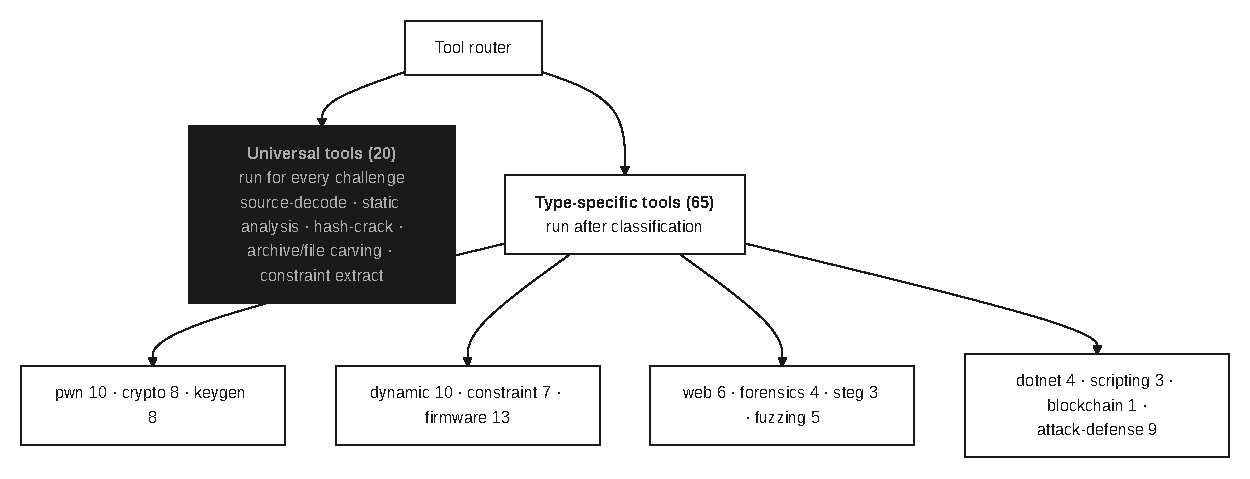
\includegraphics[width=0.98\linewidth]{figures/fig_taxonomy.pdf}
  \caption{The 85-tool library. Universal tools (in black) run deterministically for every challenge;
  type-specific tools run per category after classification.}
  \label{fig:taxonomy}
\end{figure}

\begin{table*}[t]
  \centering\small
  \setlength{\tabcolsep}{7pt}\renewcommand{\arraystretch}{1.25}
  \begin{tabular}{@{}l r >{\ttfamily\raggedright\arraybackslash}p{0.70\linewidth}@{}}
    \toprule
    \textbf{Category} & \textbf{n} & \normalfont\textbf{Representative tools} \\
    \midrule
    constraint      & 7  & auto\_angr, auto\_angr\_advanced, auto\_z3\_decompile, auto\_gdb\_cmp \\
    crypto          & 8  & auto\_rsa\_attack, auto\_lattice\_attack, auto\_padding\_oracle, auto\_prng\_crack \\
    keygen          & 8  & auto\_angr, auto\_c\_brute, auto\_c\_rand, auto\_patcher \\
    dynamic         & 10 & auto\_gdb\_solve, auto\_dynamic\_trace, auto\_memory\_dump, auto\_vm\_analyze \\
    dotnet          & 4  & auto\_angr, auto\_deobfuscate, auto\_z3\_decompile, auto\_patcher \\
    pwn             & 10 & auto\_pwn\_solve, auto\_heap\_exploit, auto\_rop\_extract, auto\_libc\_lookup \\
    forensics       & 4  & auto\_pcap\_extract, auto\_steg\_extract, auto\_file\_carve, auto\_forensics\_advanced \\
    steg            & 3  & auto\_steg\_extract, auto\_file\_carve, auto\_forensics\_advanced \\
    fuzzing         & 5  & auto\_angr, auto\_angr\_advanced, auto\_fuzz\_harness, auto\_patcher \\
    web             & 6  & auto\_web\_exploit, auto\_graphql\_exploit, auto\_jwt\_crack, auto\_webhook\_oob \\
    firmware        & 13 & auto\_firmware\_recon, auto\_dwarf\_structs, auto\_ingress\_contracts, auto\_patch\_synth \\
    scripting       & 3  & auto\_vm\_analyze, auto\_process\_interact, auto\_pyjail \\
    blockchain      & 1  & auto\_solidity\_exploit \\
    attack\_defense & 9  & auto\_exploit\_deployer, auto\_service\_keeper, auto\_tick\_orchestrator, auto\_ad\_client \\
    \bottomrule
  \end{tabular}
  \caption{The fourteen type-specific tool categories with real per-category counts from the manifest
  (representative tools shown; the full membership is in the manifest). Twenty universal tools and five remote
  tools sit alongside these; 85 tools are registered in total.}
  \label{tab:categories}
\end{table*}

\begin{table*}[t]
  \centering\small
  \setlength{\tabcolsep}{6pt}\renewcommand{\arraystretch}{1.18}
  \begin{tabular}{@{}l l p{0.50\linewidth}@{}}
    \toprule
    \textbf{Helper} & \textbf{Domain} & \textbf{What it does} \\
    \midrule
    \code{auto\_pwn\_solve}     & binary exploitation & thirteen exploit strategies (ret2win, ret2libc, ROP, SROP, one-gadget, and more), tried in order \\
    \code{auto\_angr\_advanced} & symbolic execution  & seven enhancements over base angr: state pruning, libc hooks, backward and veritesting modes, timeout recovery \\
    \code{auto\_crypto}         & classical crypto    & RC4, AES, CBC bit-flipping, CTR nonce reuse, hash length extension, ECB byte-at-a-time oracle \\
    \code{auto\_ghidra\_recover}& reverse engineering & headless Ghidra decompilation to annotated C, preserving an importable project artifact for handoff \\
    \code{auto\_steg\_extract}  & steganography       & eleven methods: LSB, EXIF, binwalk, appended-data carving, per-channel and multi-plane analysis, audio steg \\
    \code{auto\_forensics\_advanced} & forensics      & memory, disk, registry, browser, and email artifact analysis \\
    \code{auto\_deobfuscate}    & anti-analysis       & UPX unpacking, string decryption, control-flow unflattening \\
    \bottomrule
  \end{tabular}
  \caption{Flagship helpers. Each is a standalone executable obeying the same stdout contract; the
  router shells out and reads \texttt{EXTRACTED FLAG:}. The library is hot-pluggable, so a new helper is a
  one-line manifest edit rather than a code change to the graph.}
  \label{tab:helpers}
\end{table*}

\section{The Solve Engine}
\label{sec:solve}

When the deterministic cascade stalls, the solve engine is the first place a model does real work. It is
an LLM-high node running a generate, execute, fix inner loop, by default one generation plus up to three
fixes. The strategy timeout scales with the challenge type (300 seconds for constraint and fuzzing where
angr is slow, down to 30 for keygen).

The engine is opinionated about the code it accepts. A \emph{script contract} strips banned network
imports, parses the source, auto-wraps it into a \texttt{main()} with a guard, enforces a 260-line limit,
rewrites every \texttt{chr(x)} to \texttt{chr(x \& 0xFF)} through an AST transformer so an off-by-range
byte never crashes the script, and appends a \texttt{print} of the flag if the code produced none. When a
run fails on a missing module, the engine reads the \texttt{ModuleNotFoundError}, pip-installs the package
(mapping friendly names, so \texttt{Crypto} becomes \texttt{pycryptodome} and \texttt{pwn} becomes
\texttt{pwntools}), and re-runs, up to twice.

Two guards keep it honest. First, \emph{false-positive detection}: a script that exits zero with output
is not trusted blindly; if the output carries failure signals (``unsat'', ``no solution'', a traceback) a
sentinel is fed into the next fix iteration rather than declaring victory. Second, the \emph{flat-Z3 mode}:
when small models repeatedly fabricate plausible-but-wrong transformation arrays and loop on
\texttt{IndexError}s, the engine detects two or more such signatures in the last four attempts and forces a
deterministic flat solver mode that bans the offending indexed-lambda patterns outright. This is a fix that
turns a model failure mode into a policy.

\section{The Flag Validator: the Oracle}
\label{sec:validator}

Nothing counts as a solve until the deterministic validator accepts it, which is what keeps an autonomous
system from confidently reporting non-flags. The validator carries seventeen common flag-format patterns
(picoCTF, flag, uiuctf, HTB, CSAW, DUCTF, TUCTF, and others), each of the form \texttt{prefix\{...\}}, plus
four broad fallback patterns for when a challenge supplies an invalid regex, and it also checks five common
output-file locations.

Around those patterns sits a layer of noise and hallucination defense. About forty runtime-noise prefixes
(Rust, LLVM, DWARF, Go, glibc, ELF, and build-tool tokens) are rejected outright, so a mangled symbol never
passes as a flag. A low-diversity heuristic rejects bodies that are a single repeated character or, for
longer bodies, fall below a character-diversity ratio, while still keeping legitimate binary and hex flags.
A printability check requires every byte in range. Most importantly, a hallucination detector rejects a
hardcoded flag literal in a script unless the script shows real computation indicators (a subprocess,
angr, z3, pwntools), and a hallucination-loop guard escalates to the manager when the same rejected flag
reappears. For native ELF targets, a candidate can be fed back to the binary as stdin and cross-checked
against the program's own positive and negative responses, which is how planted red-herring strings are
caught.

\section{The Manager and its Eight Guards}
\label{sec:manager}

When a tier fails, control returns to a strategic manager. The important detail is that the manager is not,
in the first instance, a model call. Before it ever proposes a new strategy with an LLM it runs eight
deterministic guards (Table~\ref{tab:guards}), preceded by hard budget terminators (at most five
strategies, six hundred steps, and twenty solve attempts). Thrash detection here is policy, encoded in
state checks, not a heuristic buried in a prompt. Only if the guards pass does the manager make its one
LLM-high structured call, and even then a \emph{strategy-diversity hint} tells the model which categories
are overused and which are untried. If the model fails to parse, the manager defaults to giving up rather
than looping.

\begin{table}[t]
  \centering\small
  \setlength{\tabcolsep}{5pt}\renewcommand{\arraystretch}{1.18}
  \begin{tabular}{@{}l p{0.60\linewidth}@{}}
    \toprule
    \textbf{Guard} & \textbf{What it catches} \\
    \midrule
    Loop detection    & repeated node, script-hash, or output cycles (three sliding windows) \\
    Strategy diversity & overused categories versus untried ones, injected into the prompt \\
    Contract-thrash   & repeated solve-engine contract errors; gather artifacts instead \\
    No-output-thrash  & repeated exit-zero, empty-output runs; escalate the specialist \\
    Error persistence & repeated \texttt{IndexError}s force a flat-Z3 solver mode \\
    Stall-breaker     & repeated route-to-solve-engine actions force a specialist pivot \\
    Helper pivot      & Z3 transcription crashes climb a helper ladder (angr, c\_brute, regex\_z3) \\
    Extraction pivot  & repeated unsat climbs angr, brute-force, then a fundamentally different strategy \\
    \bottomrule
  \end{tabular}
  \caption{The eight deterministic guards the manager runs before any LLM-high strategy call, plus hard
  budget terminators. Each is a policy check on state.}
  \label{tab:guards}
\end{table}

\section{The Learned-Experience Optimizer}
\label{sec:learn}

The property that most distinguishes \kraken{} from both prior lines is that it gets better at ordering its
own work. A closed-loop optimizer records the outcome of every solve and feeds it back into the cascade
(Figure~\ref{fig:learned}). After each session a performance database accumulates per-tool statistics,
runs, successes, and timing, broken down by challenge type, with a careful attribution rule: a tool is
credited with a success only when it is the tool that actually produced the accepted flag. A failure
taxonomy records why a tool did not produce a flag, across eight failure types (no tool match, partial,
wrong classification, flaky model, timeout, crash, rejected flag, unknown).

From those, the optimizer regenerates a learned cascade configuration once a type has at least five
samples. The ordering is a composite score, \emph{success rate times one thousand plus a speed term}, so
any tool that has ever solved a type floats to the front and faster tools break ties. A tool with zero
successes after at least eight runs is dropped, though a safety valve never lets a cascade shrink below
three tools. Per-tool timeouts are tuned to the ninety-fifth percentile of observed runtimes times 1.3,
clamped to a sane range. The router loads this configuration on the next solve, appends any newly
registered tools the config predates, and falls back silently to defaults if the file is absent, so a cold
start is never broken. The result is that the cheapest-first cascade becomes cheapest-first \emph{for the
challenges this deployment actually sees}, a form of learning that costs no model calls and produces an
auditable JSON artifact rather than an opaque weight update.

\begin{figure*}[t]
  \centering
  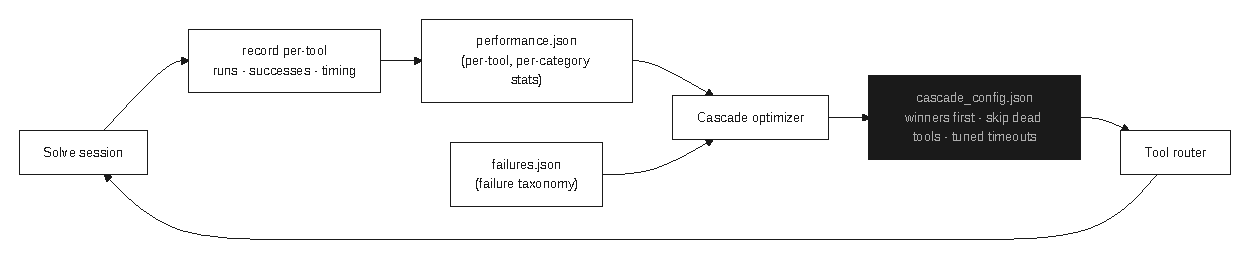
\includegraphics[width=0.92\linewidth]{figures/fig_learned.pdf}
  \caption{The learned-experience loop. Every solve updates per-tool statistics (\texttt{performance.json})
  and a failure taxonomy (\texttt{failures.json}); the optimizer regenerates a cascade configuration (in black,
  \texttt{cascade\_config.json}) that the router loads on the next solve.}
  \label{fig:learned}
\end{figure*}

\section{The Model Layer and the Codex Rescue Seat}
\label{sec:models}

\textbf{Three tiers, one interface.} Every node that needs a model calls a single \code{direct\_generate}
interface with a tier: low, mid, or high. By default the high and mid tiers are Opus and the low tier is
Sonnet, driven through the \texttt{claude} command-line tool on a Max subscription with no API key. The tier
assignment is fixed: the manager and solve engine are high, the specialists are mid, and normalize,
classify, and the context compressor are low.

\medskip
\textbf{Model-agnostic by design.} The point of the single interface is that the graph is a harness, not a
wrapper around one model. The only thing that changes between a frontier run and a local run is one backend
setting: with the Ollama backend, \code{direct\_generate} talks to a local model server, the runtime assigns
pulled models to tiers, and an access or authentication error transparently reroutes to the local model. The
graph, the prompts, and the tier calls are byte-for-byte identical. This is what makes the deterministic-tier
benchmarks runnable offline at zero cost, with no data leaving the machine.

\medskip
\textbf{How the model choice evolved.} \kraken{} started on local models, but I pivoted to frontier
models quickly, because as the complexity of the CTF problems grew I simply needed them; so I invested in a
Claude Max subscription and an OpenAI Codex subscription. Part of the reason was a design worry worth stating
plainly. If a strong frontier model writes the solves and scripts, it overfits the harness to what that model
produces, and a weaker local model can then coast in and crumble the moment it meets a challenge it has never
seen. The decision process I wanted was the rigorous one: ``I have never seen this before, so I should write
something new and add it to the repertoire.'' You cannot expect a 20-billion-parameter local model to invent a
novel script for a hard CTF problem, but you can build a harness that recognizes the novelty, reaches for the
capable model to write the new tool, and then keeps that tool. The direction I prefer, then, is a genuinely
model-agnostic harness whose deterministic tooling and routing carry the solve, so the harness \emph{guides}
whatever model is behind it toward a flag rather than depending on a particular one. The offline, zero-cost
mode is real and is how the deterministic-tier numbers were measured; it is a capability of the harness, not a
claim that every run was free.

\medskip
\textbf{Claude Code, two senses.} Claude Code drives \kraken{} in two ways. As a backend, each node's model
call shells out to \texttt{claude -p} as a single-turn generator. As a runtime, the MCP server
(Section~\ref{sec:platform}) exposes the deterministic tooling and Claude Code is the agent that invokes it,
which is the mode used in modern production runs.

\medskip
\textbf{The Codex rescue seat.} Codex is not model racing; it is an agentic strategy pivot. When the
structured pipeline exhausts its solve attempts (the default is twenty) without a flag, and before giving
up, the manager can hand the whole challenge directory to Codex as an independent agent that reads files,
writes scripts, executes them, and iterates, a fundamentally different loop from \kraken{}'s
generate-one-script-and-run approach. It fires at most once per challenge, guarded by a state flag and a
tunable threshold, and only when explicitly enabled and \texttt{codex login} has been run (a subscription
seat, no per-call billing). Before invoking it, \kraken{} dumps its own analysis (decompiled C, binary
info, strings, extracted parameters, and the current hypothesis) into a scratch directory so Codex starts
with full context. Codex is chosen deliberately because it is a different model family and so acts as an
adversarial second opinion with full file access and no graph constraint. The same seat is available
interactively in a Claude Code session as \code{codex:rescue} for manual investigation of a stuck challenge.

\section{Beyond Jeopardy: Attack-Defense}
\label{sec:ad}

CTF is not only jeopardy solving. In an attack-defense competition every team runs the same set of
services, and each tick a team must both attack the other teams (find a bug, exploit it across the field,
submit the captured flags) and defend its own services (detect incoming exploits, patch, and keep the
service available). \kraken{} supports both sides. One caveat up front, stated honestly: the catch-and-throw
attack-defense integration is newer and less battle-tested than the jeopardy path, built and unit-tested but
not yet proven across a full live competition. It is described here as an architecture, not a track record.
There are nine attack-defense
helper tools that serve as command-line building blocks, and above them a dedicated tick engine (about
6{,}400 lines) that orchestrates a full round. Each tick runs four phases concurrently, offense, defense,
service-level-agreement checking, and scoreboard update (Table~\ref{tab:ad}).

\medskip
\textbf{The throwing side.} Each tick, the engine builds a task for every opponent team crossed with every
service and runs them under a concurrency limit, so a single discovered bug is mass-thrown across the whole
field. Captured flags are submitted immediately through an async, deduplicated, rate-limited submitter that
classifies each scorebot reply (accepted, duplicate, expired, own-flag, rejected) and never resubmits a
flag. Exploits are hot-reloaded from disk every tick and pruned automatically when their success rate
drops below five percent. The bridge from the jeopardy solver into this mode is direct: a
\code{kraken\_full\_solve} result, or a static vulnerability finding, is turned into a standalone pwntools
exploit script (ret2win, ret2system, shellcode, format-string, heap, or ROP templates) and deployed.

\medskip
\textbf{The catching side.} The defensive pipeline analyzes the previous tick's packet capture, matching
shellcode signatures, format-string payloads, and De-Bruijn cyclic overflow patterns to detect incoming
attacks. For each detected attack it can auto-patch its own service (a bounds check for an overflow, a
\texttt{printf("\%s", buf)} rewrite for a format string) and, critically, it validates the patch against
the SLA monitor and rolls back if the patch breaks the service. Detected incoming attacks are also replayed
and, when they verify, converted into the team's own throwers, so an opponent's exploit becomes yours.
Dynamic firewall rules block payload signatures and repeat-offender source addresses in a dedicated iptables
chain that whitelists the SLA checker. A service-keeper helper adds snapshot-and-restore, detecting file
integrity drift, a downed service, or process injection and restoring clean state.

\begin{table}[t]
  \centering\small
  \setlength{\tabcolsep}{5pt}\renewcommand{\arraystretch}{1.18}
  \begin{tabular}{@{}l p{0.62\linewidth}@{}}
    \toprule
    \textbf{Phase} & \textbf{Per-tick action} \\
    \midrule
    Offense   & mass-throw every exploit at every opponent service under a concurrency limit; submit captured flags immediately; prune exploits below 5\% success \\
    Defense   & sniff the prior pcap for shellcode, format-string, and cyclic-overflow payloads; auto-patch with SLA-gated rollback; replay captured attacks into your own throwers; install dynamic firewall blocks \\
    SLA       & probe every service; log any that are down \\
    Scoreboard & poll the game protocol (Faust, iCTF, Nautilus, or generic) for standing and tick boundary \\
    \bottomrule
  \end{tabular}
  \caption{The attack-defense tick engine runs four phases concurrently each tick. Offense turns one bug
  into a field-wide flag harvest; defense detects, patches, self-heals, and steals back.}
  \label{tab:ad}
\end{table}

\section{The Wider Platform}
\label{sec:platform}

\kraken{} is a platform, not a single entry point. The pieces below all sit on the same graph and library.

\medskip
\textbf{MCP server (30 tools).} A FastMCP server exposes the deterministic tooling over stdio so an
external agent, typically Claude Code, can drive it: triage, decompile, parameter extraction, single-tool
and full-cascade runs, flag validation, script execution, timing and remote interaction, ELF repair,
disassembly, a one-shot \code{kraken\_full\_solve}, plus reporting, retrospective, knowledge query, and
performance and failure statistics. The server itself makes no LLM calls; the intelligence is the agent
driving the tools.

\medskip
\textbf{Live-competition autopilot, and combined execution.} A CTFd client authenticates, pulls every
challenge in a competition, builds a workspace for each, and submits flags under a deliberately conservative
policy: only a high-confidence flag is submitted, exactly once per challenge, with no brute-force and no retry
on ``incorrect.'' The mode that ties the whole system together is what I call combined execution: pull all the
challenges at once, then dispatch one agent per challenge in a single wave under a concurrency semaphore, and
let each agent independently run the entire graph on its own challenge, intake, classification, the selected
label, routing to a specialist, the tool cascade, and the validator. A monitor mode watches for newly released
challenges and folds them into the wave; a dry-run mode solves without submitting. The BYU EOS run in
Section~\ref{sec:practice} is exactly this: 42 agents dispatched in one message, one per challenge, each
running the full pipeline in parallel, the whole board cleared in about ten minutes.

\medskip
\textbf{Batch solving and the GUI.} A \code{solve-all} runner solves a whole directory of challenges in
parallel. A FastAPI browser GUI exposes the pipeline over REST with WebSocket streaming of live solve
progress, backed by a background job store.

\medskip
\textbf{Sandboxing, artifacts, and ledgers.} \kraken{} can optionally run a challenge binary inside an
isolated Docker container for safety; this is distinct from the ``non-Docker'' benchmark subsets discussed
in Section~\ref{sec:eval}, which are challenges that do not require a live networked instance. A handle-based
artifact store keeps large binary data (decompilation, angr results, traces) out of the graph state, shrinking
checkpoints from hundreds of kilobytes to a few hundred bytes, and a post-solve artifact bundle emits a
per-challenge summary, a tool-cascade log, a knowledge-graph file, and a standalone \code{reproduce.sh} for
handoff and audit. Two ledgers coexist: a per-challenge scratchpad that redacts flag-like tokens before
persisting, and a shared SQLite case-state ledger that gives the helpers and a sister vulnerability-research
agent a common memory.

\section{Testing and Quality}
\label{sec:tests}

\kraken{} ships with \textbf{1{,}037 tests} and, by deliberate choice, \textbf{no continuous integration};
there is no \code{.github} directory at all. The suite is heavily biased toward deterministic, offline units:
the parameter extractor, the classifier heuristics, the flag validator, the tool router, and the failure
taxonomy are all tested without a single model call, using mocks. The flag validator has golden-flag tests
that assert not only that real flags are accepted but that flags embedded in comments, regexes, and
format-strings are \emph{rejected}. The attack-defense engine alone carries 134 tests. The suite honestly
records its own gaps: two strict-\code{xfail} tests document that nineteen older helper scripts predate the
\code{tool\_meta.json} registry and are not yet registered, a real coverage gap left visible rather than
hidden, and the benchmark and regression suites were physically removed for the public snapshot rather than
left as dead weight. The philosophy is the same one that governs the runtime: prefer the deterministic thing,
and be honest about what is not yet covered.

\section{In Practice: What It Actually Solved}
\label{sec:practice}

Benchmarks are a floor, not the story. The story is what \kraken{} did against real challenges, in real
competitions, in the agent's own words.

\begin{finding}{The doubtful challenge author}
At KalmarCTF 2026, the challenge author of a 1000-point reverse-engineering problem (\texttt{flag\_checker},
zero solves at release) shipped a single artifact: a 135\,KB bitstream for a Lattice iCE40 HX8K FPGA. The
prompt was only ``iCE40 HX8K EVB, 9600 baud, make the led light up.'' The flag lived in the hardware.
\kraken{}'s agent converted the bitstream to a Verilog netlist with the Project IceStorm tools, found that an
internal signal (\texttt{n226}) pulses on each correct character, built an Icarus Verilog testbench driving the
UART at 9600 baud, and brute-forced the flag one position at a time: all 95 printable ASCII characters in
parallel per position, about five minutes per position across 92 positions, roughly eight hours and fully
autonomous. Two positions fought back, and the agent adapted: at position 18 the match signal stuck high and
needed a filtered detector, and at position 85 it stopped incrementing and needed an alternative counter. The
part that stays with me is what the recovered flag actually said. It was not the usual jumble of
underscores; it was a full English sentence, and the sentence was the author's own bet, written into the
answer, that this simple reverse-engineering challenge could not be solved by an AI. It was, one character at
a time, through eight hours of hardware simulation.
\end{finding}

\medskip
\textbf{More from the same competition.} KalmarCTF was an anti-AI event, and the team (one human plus a
Claude-driven agent) played less than half of the competition time, running out of tokens because I started
the week with less than half of my model allowance left after other project development, yet still placed 26th
of 275 (top ten percent) and produced solves across a striking range.
It wrote a ring-0 kernel exploit on a hobby OS in about thirty minutes: install a call gate in the LDT,
reload the LDT register through a fork, far-call to ring 0, and use a ROP chain to replace the filesystem's
authorization listener with a function that always returns granted, then read the flag. It recovered a
neural network's weights from a black-box oracle by gradient peeling, an ultra-fine scan locating all 128
ReLU breakpoints and reconstructing the weight matrix in roughly 55{,}000 queries and forty minutes. It
broke a zero-knowledge proof system's soundness by exploiting that a sigma protocol's constraint was only
two-special-sound. It found and exploited a genuine, previously unreported path-traversal vulnerability in
CTFd 3.8.1 (a double-slash archive-import that yields arbitrary file write, fixed upstream in 3.8.2). And it
solved a challenge of 3{,}500 XORed LFSRs by computing a degree-6.8-million product tree and decomposing it
into partial fractions, after fixing a subtle bug in a GF(2) formal-derivative routine that cut a step from
162 seconds to under a tenth of a second. These are solves across kernel exploitation, machine learning,
cryptography, and web, not a narrow strength.

\medskip
\textbf{A fast, near-total clear.} Where the challenges fit \kraken{}'s wheelhouse, the story is speed and
completeness. At the BYU End-of-Semester CTF~2026 the harness pulled all 43 challenges from CTFd, locked the
flag format, and dispatched 42 agents in a single message, one per challenge, each with the full MCP
toolchain. It solved every challenge that was solvable online, 39 of 42, in a single wave of about ten
minutes. This was done completely remotely, and three of the challenges required being physically present to
solve, so while in spirit I finished first, in reality I most likely landed among the top few competitors once
everything was said and done. What matters for this report is not the placement but that BYU EOS was an
excellent testbed for autonomous auto-solving, and the wave cleared the entire online-solvable set hands-off.

The breakdown of that wave is more useful than a clean headline: in about ten
minutes of wall clock the agent correctly and autonomously solved 18 new challenges (20 counting two already
solved on pull), submitting 18 of 21 under a strict one-attempt-per-challenge rule, with one
informed-but-wrong OSINT guess that was not retried. The challenges it did not close were not failures on
tractable digital problems; they were blocked by offline remote infrastructure, physical or attendance
gating, or API policy refusals (Section~\ref{sec:didnt}). Among the clean solves, one reverse-engineering
flag, recovered from about 7{,}000 dot-functions forming a linear byte-op chain, literally read
\texttt{byuctf\{i\_hope\_u\_used\_angr\}}; the agent had done it the hard way and still nailed it. Others
ranged from an AES-GCM forbidden-attack cookie forgery to a JPEG-plus-ZIP polyglot to a blind-XSS admin-cookie
exfiltration. A comprehensive worked example of the \texttt{flag\_checker} solve, with artifacts, lives in
the private development tree.

\medskip
\textbf{Attack-defense and embedded firmware.} The expansion beyond jeopardy is not theoretical. At MITRE's
Embedded CTF, a year-long embedded attack-defense competition where every team builds a hardware security
module on a fixed TI MSPM0L222x (a Cortex-M0+ with 32 KB of RAM and 256 KB of flash), \kraken{} broke down a
target firmware (about 3{,}700 lines of C statically linked with wolfSSL) in about ten minutes of core
analysis. Driven through the \code{/triage}, \code{/decompile}, and \code{/postmortem} commands, it found a
\code{read\_packet} length-check bypass (a bound parameter initialized to zero short-circuits the check and
lets an attacker declare a 65-kilobyte length), a single global stack canary at a fixed address (forgeable
because there is no per-function randomization), and a ROP path into the firmware's own \code{write\_bytes}
routine to dump the file store back over the UART. Because the firmware shipped unstripped with DWARF, the
``decompile'' step reduced to a source lookup rather than a cold Ghidra run, which the agent measured as
roughly a thirty-fold speedup. It even noticed, and dismissed within thirty seconds, a planted magic string
designed to spook an AI attacker into refusing. This run is also where the honesty is sharpest
(Section~\ref{sec:lessons}): the agent documented exactly where it broke down, and those gaps became the
thirteen firmware-category tools the system now ships.

\section{Evaluation}
\label{sec:eval}

\textbf{Methodology, stated plainly.} A solve counts only when the deterministic flag validator accepts the
flag. There is no partial credit, no self-report, and no human confirming a model's guess: the same oracle
that gates the pipeline gates the score (Section~\ref{sec:validator}). Benchmark subsets are disclosed rather
than quietly chosen. The offline runs use the \emph{non-Docker} subsets, meaning challenges that do not
require a live networked instance. That subset is exactly the static class the cascade targets, and by the
same token it excludes the interactive class the cascade is weak on (Section~\ref{sec:lessons}). Stating the
subset is the point: it draws the boundary of the claim instead of inflating it. Table~\ref{tab:eval}
collects the results that have a scoreboard or a deterministic oracle behind them.

\begin{table*}[t]
  \centering\small
  \setlength{\tabcolsep}{7pt}\renewcommand{\arraystretch}{1.5}
  \begin{tabular}{@{}p{0.17\linewidth} p{0.10\linewidth} p{0.14\linewidth} p{0.135\linewidth} p{0.315\linewidth}@{}}
    \toprule
    \textbf{Setting} & \textbf{Scale} & \textbf{Result} & \textbf{Adjudication} & \textbf{Evaluation} \\
    \midrule
    BYU EOS CTF 2026 & 42 challenges & 39/42 online-solvable & online \mbox{(frontier)} & cleared every online-solvable challenge hands-off; I asked to be removed from the leaderboard, so a top finish in spirit, not an official placement \\
    KalmarCTF 2026 & 275 teams & top 10\% (26th) & online \mbox{(frontier)} & an anti-AI event; played less than half of the competition time, out of tokens (started the week with under half my model allowance after other project work) \\
    \mbox{CTFTiny} \mbox{(non-Docker)} & 23 challenges & 23/23, 21 at zero tokens & offline \mbox{(Ollama)} & the static subset; the one setting measured on a local model, so a clean read on the deterministic tier \\
    MITRE eCTF \mbox{(DSU firmware)} & 1 target & full breakdown, $\sim$10 min & online \mbox{(frontier)} & an analysis pass, not a scored round; the ``where it broke down'' section drove 13 new tools \\
    Cumulative (all settings + practice) & hundreds solved & validator-confirmed & online \mbox{(frontier)} & most serious runs used frontier models on a paid subscription; only the CTFTiny row was measured offline (Ollama) at \$0 \\
    \bottomrule
  \end{tabular}
  \caption{Results with a scoreboard or a deterministic oracle behind them. Every figure is a
  validator-accepted flag, not a self-report; every subset is disclosed. The CTFTiny row measures the
  deterministic tier in isolation; the KalmarCTF row measures the frontier tier on the class the cascade
  cannot reach alone.}
  \label{tab:eval}
\end{table*}

The two extremes in Table~\ref{tab:eval} are the honest bracket of the whole design. CTFTiny is the best
case: a static subset the deterministic tier clears completely, 21 of 23 without spending a single model
token. KalmarCTF is the hard case: an anti-AI event whose interactive challenges the cascade alone cannot
reach, where the frontier tier does the work and the runs were paid. A system that reports both, rather than
only the favorable one, is telling the reader where it actually stands.

\section{What Did Not Work}
\label{sec:didnt}

Our results were not all good. This took time: iteration, improvement, expansion, and design. Valuable
testbeds like the BYU EOS CTF pushed the system hard, and even there we ran into problems, hiccups, and
nuances. The system is robust, but it is not perfect, and to expect it to run perfectly every time would be to
set yourself up for disappointment. So it is worth getting into where it fell short. The BYU run is a good
teacher precisely because a large fraction of the challenges the agent did not close failed for reasons worth
naming, and none of them were ``the model could not reason about it.''

\medskip
\textbf{API policy refusals.} Four of the five Git challenges were never even read: the generic solver agents
tripped a safety classifier because the task framing (``find secrets in a git repo,'' ``search for
credentials'') pattern-matched onto something the classifier dislikes when it is not explicitly labeled as a
sanctioned exercise. The lesson, encoded afterward, is twofold: keep dispatched instructions high-level and
concept-level rather than listing exact incantations (in a second pass, \emph{more} specific prompts refused
\emph{more} reliably, and even flipped two previously-successful challenges to refused), and build a dedicated
git-forensics helper whose framing is unambiguously a sanctioned CTF exercise so the agent-framing problem
disappears entirely.

This refusal friction, a capable model declining a sanctioned exercise because of how the task was worded, is
also what set me down a parallel line of work: the framing and robustness of those safety boundaries
themselves. That effort became a jailbreak-focused sister project, \texttt{project\_wraith}, which will get its
own paper the way \texttt{project\_blackbox} will.

\medskip
\textbf{Remote infrastructure offline.} Four PWN exploits were written, verified against local replicas, and
then had nowhere to fire because the live remote service was down for the window. These are correctly labeled
``exploit verified, remote pending,'' not ``failed'': an OOB negative-index leak, a signed-index GOT
overwrite, a 32-bit integer-overflow price wrap, and a two-stage ret2libc were all production-ready. The fix
is an upfront remote-availability probe in triage so a down service is tagged and routed to the
local-verification path rather than counted as a solve failure.

\medskip
\textbf{Physical and attendance gating.} Several challenges required a real floppy disk read on campus, a flag
handed out at a live event, or a kiosk interaction. There is no digital path, and the honest response is to
detect them (a physical-challenge classifier keyed on ``in-person,'' ``on campus,'' ``floppy,'' ``attend'')
and fast-fail immediately instead of burning ten minutes of agent time, which is exactly what the earlier run
did wrong.

\medskip
\textbf{Budget and tooling gaps.} One reverse-engineering challenge, a 1{,}817-op signal-driven tape VM, was
correctly reverse-engineered but did not finish its symbolic solve inside the ten-minute budget. One OSINT
challenge was narrowed from sixteen candidate buildings to six but was ultimately blocked because the agent
had no reverse-image-search tool and the decisive placard was unreadable at source resolution. These are
honest capability gaps, not reasoning failures, and they point directly at the roadmap.

\medskip
\textbf{The second-pass system.} The most useful artifact of documenting these failures is a second-pass
orchestrator built afterward. It keeps a state machine over every challenge (solved, already-submitted-incorrect,
physical, remote-offline, timed-out, tool-missing), never re-touches a validated solve, honors the
one-attempt-per-challenge rule idempotently, and fast-fails the remote-offline class in seconds rather than
minutes. On a re-run it captured zero new flags, and that null is itself the result: it proved the remaining
challenges were genuinely blocked on infrastructure, physical access, or missing tools, not on solver
capability, and it carried real work forward (a hand-built VM simulator and a fast signal oracle) as concrete
tickets for a third pass. A null from a disciplined instrument is a finding.

\medskip
\textbf{Under-represented categories, and the new obstacles.} The deepest limitation is simply coverage: the
engine is only as good as what it has seen and what I prepared it for. But it also learns from experience
(Section~\ref{sec:learn}), which is exactly the argument for exposing it to as many different testbeds and
competitions as possible, so its repertoire grows. The harder trend is what the newest events are doing on
purpose. In this emerging age of anti-AI CTF, more challenges lean on heavy manual configuration or obscure
setups, up to and including full virtualization platforms like VMware or QEMU, precisely because that
friction stops an autosolver. I do not think that is a bad thing for the competitions, but it does pose
the real research question for a system like this: can you give the agent all the resources and guidance it
needs to work through those environments too, and at what point does that become tractable through browser-use
and computer-use rather than a fixed tool cascade? That path has its own concerns. My own view is that any
agent operating at that level of access should run inside a containerized, sandboxed platform, which is
correct for safety but adds a whole new layer of orchestration complexity to the problem. It is squarely
future work, and it is where the interesting part now lives.

\section{Impact and Significance}
\label{sec:impact}

Across benchmarks, historical challenges, and live competitions, \kraken{} has autonomously solved hundreds
of CTF challenges. But the raw count is not the significance.

\medskip
\textbf{Why this matters beyond CTF.} A CTF challenge is a compressed, graded proxy for a real security task,
which is what makes an autonomous CTF system more than a game player. Each capability the cascade exercises has
a direct operational analogue (Table~\ref{tab:beyond}). Reversing a stripped binary is the core loop of malware
and firmware analysis, and the eCTF run is precisely that loop on real embedded firmware. Triggering and
exploiting a memory bug is vulnerability discovery with a proof of concept attached. Classifying an unknown
artifact with no signature is exactly the triage problem for a novel threat. The autosolver is a way to build
and measure those capabilities against an oracle that cannot be argued with.

\begin{table*}[t]
  \centering\small
  \setlength{\tabcolsep}{6pt}\renewcommand{\arraystretch}{1.2}
  \begin{tabular}{@{}p{0.42\linewidth} p{0.50\linewidth}@{}}
    \toprule
    \textbf{CTF capability} & \textbf{Operational equivalent} \\
    \midrule
    Reverse a stripped binary or firmware image & malware and firmware analysis \\
    Trigger and exploit a memory-safety bug     & vulnerability discovery with a proof of concept \\
    Break weak or misused cryptography          & protocol and key-handling audits \\
    Recover model internals from a black box    & model-extraction and ML-security assessment \\
    Defend and self-heal a live service         & incident response and automated patching \\
    Classify an unknown artifact with no signature & triage of a novel threat \\
    \bottomrule
  \end{tabular}
  \caption{The autosolver as a capability instrument. Each CTF task the cascade performs maps onto a real
  defensive or research task, measured against a deterministic oracle rather than a subjective score.}
  \label{tab:beyond}
\end{table*}

Two further properties give the design significance the solve count does not capture. The first is
\textbf{economic potential}. Because the deterministic tier can close a challenge with no model call, the
design's cost is meant to scale with \emph{difficulty} rather than \emph{volume}: cheap challenges cost
nothing, and paid inference is reserved for the hard tail. This is a property of the architecture, not a
claim about the runs in this report, most of which used a paid frontier subscription; realizing the low-cost
promise at scale is future work, and a reason to keep the harness model-agnostic so cheaper open-weight models
can carry more of the load. The second is \textbf{auditability}. A deterministic solve is a reproducible artifact: the same
inputs yield the same flag and the same trace. The validator oracle means the system never reports a non-flag
as a win, and the learned configuration is a human-readable file rather than an opaque weight update. In any
setting where a result must be justified to someone else, a graded assessment, a disclosure, an audit, ``here
is the byte-for-byte trace'' is a stronger claim than ``the model said so.'' That auditability is what makes
the approach portable to the sister vulnerability-research agent, where a finding is only useful if it can be
reproduced and defended.

\section{Lessons Learned}
\label{sec:lessons}

\textbf{The static/interactive boundary is real and structural.} The cascade dominates \emph{static}
challenges (a binary to reverse, a cipher to break) and is weak on \emph{dynamic, interactive} ones (live
per-team instances, network protocols, multi-step chains). At KalmarCTF the deterministic pipeline
contributed little on the interactive challenges; the placement came from the model-driven agents. This
matches EnIGMA's finding \cite{abramovich2025enigma} that interactive tooling is what unlocks that class, and
it is exactly the tooling the cascade lacked.

\medskip
\textbf{Use the tool.} The most expensive mistake at KalmarCTF was behavioral, not architectural. Under time
pressure, generic agents were spun up that re-derived triage, decompilation, and classification from scratch
instead of invoking the pipeline that already does all of that. An autonomous system is only as good as its
own disciplined use of its strongest components.

\medskip
\textbf{Triage first, and play to strengths.} The challenges \kraken{} solved fastest were the ones a quick
triage pass would have flagged as AI-favorable up front: an FPGA to simulate, a neural network to invert, a
thousands-of-LFSRs problem to decompose algebraically. A structured read-everything-first pass beats diving
into whatever looks interesting.

\medskip
\textbf{Failures become tools, verbatim.} The system's design is the residue of concrete failures. The
constraint timeout was cut from 300 to 90 seconds after \texttt{angr} ate an entire budget on state
explosion. The crash counter and manager reroute exist because a solve-engine crash once left a stale
next-node pointer and looped on a \texttt{KeyError}. The flat-Z3 mode exists because small models fabricated
transformation arrays and looped on \texttt{IndexError}s. Most vividly, the MITRE eCTF run is where the agent
documented exactly where it broke down: pwntools found zero ROP gadgets on the ARM Thumb firmware, the
firmware specialist never fired because the classifier keyed on Linux entry symbols the bare-metal target
lacks, and \texttt{objdump} reported an unknown machine. Those seven documented gaps became the productized
firmware tools, including the ingress-contract extractor whose docstring names the very \code{read\_packet}
bug it would now catch. Honest failure analysis is the system's primary source of new capability.

\medskip
\textbf{Determinism compounds.} The deterministic short-circuit is not a micro-optimization. Solving most of a
\emph{static} set with no model call is what makes overnight, parallel, \$0 operation possible in principle,
and it is what the learned optimizer sharpens over time. And when time is of the essence, when time-to-solve
is the difference between winning and losing a challenge, a competition, or a project, an architecture that
resolves the routine work in seconds rather than model round-trips makes a real difference.

\section{Future Work}
\label{sec:future}

The roadmap follows directly from the lessons, and it is concrete because most of it is the fix for a
failure this report already named.

\medskip
\textbf{A first-class live mode.} The largest item is interactive play alongside the static path: instance
management (spawn, track expiry, reconnect, authenticate); interactive-protocol tools in the cascade itself (a
pwntools-backed connection, an HTTP client, a protocol fuzzer) rather than only in the agentic fallback; a
flag validator that can submit to a competition API; and an upfront remote-availability probe so a down
service is tagged rather than counted as a solve failure. The goal is to give the deterministic cascade the
interactive vocabulary EnIGMA showed is essential, so the tier that is fast, free, and reproducible can reach
the challenges that currently require the expensive fallback.

\medskip
\textbf{Category and tooling expansion.} The competitions made the missing categories obvious. OSINT is the
biggest single unlock: a reverse-image-search helper (wrapping the public lookup services) would open a class
the system currently cannot touch, and would have decided at least one lost challenge outright. A dedicated
git-forensics helper (deep history, reflog, dangling objects, tags, and the hosting API) both raises the git
category and, by carrying an unambiguous sanctioned-exercise framing, sidesteps the policy-refusal problem that
blocked four challenges at once. A physical-challenge classifier fast-fails attendance-gated challenges in a
second instead of ten minutes. A browser-in-the-loop web solver (headful when needed, with network
interception and a cookie jar) turns static-JS guesswork into reliable web solves, and a prompt-injection
helper prepares for the growing class of LLM-in-the-loop challenges.

More broadly, a mature reverse-engineering
autosolver wants \emph{more Ghidra scripting and more tool integrations} than it has today: deeper headless
Ghidra analyzers, more decompiler and disassembler back-ends, more binary-diff and structure-recovery passes,
and more documentation of each so the library stays legible as it grows. The bare-metal work from the eCTF run
points the same way: a dedicated bare-metal specialist and Cortex-M ROP tooling so the firmware path fires
automatically rather than through manual commands.

\medskip
\textbf{Beyond CTF platforms.} The same governed, deterministic-first engine generalizes past scored jeopardy
and attack-defense into the real-prize, domain-specific competitions that increasingly define the field:
DEF CON village-style events and hardware-and-embedded challenges in adjacent domains such as aerospace and
automotive security. These raise the bar from a graded proxy to a real target with a real payoff, and they are
exactly where a reproducible, auditable solver earns its keep.

\medskip
\textbf{Learning.} On the learning side, the per-tool optimizer generalizes naturally to cross-challenge
transfer, recognizing that a new challenge resembles a solved one and seeding the cascade accordingly, and the
outstanding nineteen-helper registry gap should be closed so the registry covers every script on disk.

\medskip
\textbf{The natural next step, and a deliberate stopping point.} There is a tension I want to name. A CTF
challenge is a graded proxy for a real security task (Section~\ref{sec:impact}), and reverse engineering and
exploitation challenges are, for many people, the on-ramp into vulnerability research. Automating that away
wholesale would take the learning opportunity out of the hands of the researchers who most need it, and I do
not want to be the one who does that. So \kraken{} is, by choice, a stopping point: the solver here has been
untouched for two to three months and is released as it stands, a complete and honest artifact rather than a
living product. What I want to realize next is this engine turned toward real-world value: augmenting
vulnerability research, and standing as the foundation to build that on. My own attention has moved along the
natural progression of AI-augmented cyber operations, toward full vulnerability-research agents: richer
disassembly, emulation, and deeper static and dynamic analysis against real targets, where the flag is a
reproducible finding and the bar is a proof of concept that survives manual validation. That is the work of
the sister project, \texttt{project\_blackbox}. The eCTF firmware breakdown in this report is the first step
across that line.

One design question matters most to me here, and its answer belongs to \texttt{project\_blackbox}'s own
writeup: how do you build an agent-based, augmented-cyber-operations system that delivers value on \emph{every}
run, bug or no bug? A vulnerability-research agent that only counts
as useful when it finds a bug wastes most of its runs. The better target is a system where each engagement,
even one that finds nothing exploitable, still produces durable value, a sharper understanding of the target,
real documentation, and reusable tooling built around it, so the next run starts further ahead. That is the
future of this work: \kraken{} as the foundation for what I am building now in \texttt{project\_blackbox}.

\section{Takeaways}

\begin{itemize}[leftmargin=1.1em,itemsep=2pt,topsep=2pt]
\item \textbf{Model-last beats model-first on the static majority of CTF work.} Spending a model only where
computation runs out is cheaper, reproducible, and offline-capable, without giving up the hard tail.
\item \textbf{A total route map plus a validator oracle is what makes autonomy safe.} No class is ever
stranded, and a non-flag is never reported as a win. Safety here is structural, not a prompt.
\item \textbf{The system is a harness, not a solver.} You direct the intelligence; the harness carries the
deterministic tooling and the routing, and guides whatever model is behind it toward a flag. Jeopardy, live
autopilot, batch, MCP, GUI, and attack-defense all run on that one graph and library.
\item \textbf{Honest failure analysis is the engine of new capability.} Nearly every guard, timeout, and
firmware tool is the fix for a documented, named failure.
\item \textbf{The result that matters is a flag, not a row in a table.} An author bet an AI could not solve his
challenge and wrote the bet into the flag; the system recovered it anyway.
\end{itemize}

\section{Conclusion}

\kraken{}'s ideology was simple. Solving a CTF challenge is, most of the time, following a methodology: a chain
of solve-notes and deterministic steps that leads to the flag. So why pay for model inference at every one of
those steps when you can guide an agent through the deterministic part and reserve the model for the moments
that genuinely need it? At runtime, most of what remains is changing a variable, running a script, or reading an
artifact the harness already produced. Do that, and you save time and money and get a cleaner solution path.
Where the problem is dynamic and interactive, the deterministic tier steps aside and frontier models, driven
through Claude Code with a Codex rescue seat, drive through it.

At the end of the day, this was an excellent project to introduce myself to the worlds of CTF, of AI and
machine learning, and to the question of how to bridge them and augment cyber operations with AI effectively.
If I am being honest, I also just wanted to prove to myself that I could, and to see for myself how far the
realm of the possible now stretches when you point AI at offensive-security work; that experiment is a good
part of what guided my decision to pursue graduate school. And nothing in the whole experience was more
validating than that single flag from KalmarCTF, the one that reads that its author did not think an AI could
solve his challenge. The first time I saw it was in the competition's postmortem, a PDF sent to me over
Discord. That was the icing on the cake.

There are still a lot of artifacts left in this project from before I pushed it to open source. If you find any
issues or errors, or have thoughts, comments, or requests, really anything at all, I would genuinely love to
hear it; I do this for the love of the game, and this was a personal passion project. My email is at the top of
this paper. Thank you for your time, and thank you for reading.

\section*{Reproducibility}

The system is in the project repository: \code{src/kraken/} (orchestrator, LangGraph assembly, the sixteen-plus
nodes, the 85-tool helper library, the attack-defense engine, runtime, and MCP server), \code{scripts/}
(including headless Ghidra helpers), \code{tests/} (1{,}037 tests), and \code{docs/} (architecture and the
offline runtime guide). The offline benchmark harness and the full per-challenge competition writeups live in
the private development tree; the figures in this report are generated from the committed architecture.

\section*{Acknowledgements}

A genuine thank-you to the other CTF autosolver teams this report compares against; the work here stands on
theirs. Squid Agent, from the SPL Team, was the direct inspiration for \kraken{}, and without it I would not
have started this at all. I am grateful to the authors of D-CIPHER, EnIGMA, HackSynth, and VeriLabs for the
ideas and for the bar they set. And none of this would exist without AIxCC, which is what first pulled me into
AI-augmented cyber operations. It is now what I do across the board.

\appendix
\section{Tool Catalog}
\label{sec:appendix}

The complete registered library is 85 tools: 20 universal, 5 remote, and 60 type-specific across fourteen
categories. The named groups below list the tools whose membership is not already given by
Table~\ref{tab:categories}; the full manifest, with per-tool command styles and timeouts, is
\texttt{src/kraken/helpers/tool\_meta.json}.

\begin{description}[leftmargin=0pt,labelsep=0.4em,itemsep=3pt,font=\normalfont\bfseries]
\raggedright
\item[Universal (20, in run order)] \ttfamily\small auto\_source\_decode, auto\_constraint\_extract,
auto\_existing\_exploits, auto\_run\_static, auto\_python\_reverse, auto\_c\_source\_eval, auto\_cpp\_compile,
auto\_qr\_decode, auto\_maze\_solver, auto\_archive\_search, auto\_git\_extract, auto\_table\_reverse,
auto\_ec\_vigenere, auto\_hash\_crack, auto\_pdf\_extract, auto\_pcap\_extract, auto\_steg\_extract,
auto\_file\_carve, auto\_substitution\_cipher, auto\_bash\_solver.

\item[Remote (5)] \ttfamily\small auto\_remote\_interact, auto\_timing\_attack, auto\_service\_interact,
auto\_process\_interact, auto\_web\_exploit.

\item[Attack-defense (9)] \ttfamily\small auto\_existing\_exploits, auto\_strip\_recover,
auto\_ingress\_contracts, auto\_patch\_synth, auto\_binary\_patch, auto\_exploit\_deployer,
auto\_service\_keeper, auto\_tick\_orchestrator, auto\_ad\_client.

\item[Firmware (13)] \ttfamily\small auto\_deobfuscate, auto\_focused\_decompile, auto\_gdb\_solve,
auto\_firmware\_recon, auto\_dwarf\_structs, auto\_memory\_map, auto\_secrets\_diff, auto\_unstripped\_decompile,
auto\_source\_structs, auto\_source\_structs\_rust, auto\_ingress\_contracts, auto\_serial\_replay,
auto\_patch\_synth.
\end{description}

{\small
\begin{thebibliography}{9}

\bibitem{squid2024}
SPL Team.
\newblock Squid Agent: a multi-agent CTF auto-solver.
\newblock SPL Team blog, \texttt{spl.team/blog/squid-agent-csaw}, 2024.

\bibitem{udeshi2025dcipher}
M.~Udeshi, M.~Shao, H.~Xi, N.~Rani, K.~Milner, V.~S.~C.~Putrevu, B.~Dolan-Gavitt, S.~K.~Shukla,
P.~Krishnamurthy, F.~Khorrami, R.~Karri, and M.~Shafique.
\newblock D-CIPHER: Dynamic collaborative intelligent multi-agent system with planner and heterogeneous
executors for offensive security.
\newblock \emph{arXiv:2502.10931}, 2025.

\bibitem{abramovich2025enigma}
T.~Abramovich, M.~Udeshi, M.~Shao, K.~Lieret, H.~Xi, K.~Milner, S.~Jancheska, J.~Yang, C.~E.~Jimenez,
F.~Khorrami, P.~Krishnamurthy, B.~Dolan-Gavitt, M.~Shafique, K.~Narasimhan, R.~Karri, and O.~Press.
\newblock EnIGMA: Interactive tools substantially assist LM agents in finding security vulnerabilities.
\newblock \emph{Proc.\ ICML}, 2025. arXiv:2409.16165.

\bibitem{muzsai2024hacksynth}
L.~Muzsai, D.~Imolai, and A.~Luk\'{a}cs.
\newblock HackSynth: LLM agent and evaluation framework for autonomous penetration testing.
\newblock \emph{arXiv:2412.01778}, 2024.

\bibitem{verialabs2026}
Veria Labs.
\newblock CTF Agent: an autonomous CTF solver that races multiple models in parallel (1st place, BSidesSF
2026).
\newblock \texttt{github.com/verialabs/ctf-agent}, 2026.

\end{thebibliography}
}

\end{document}
